% Copyright 2016 by Gokmen Goksel <gokmen@goksel.me>
% -- uses Till Tantau <tantau@users.sourceforge.net> Beamer Class

\documentclass[xcolor=dvipsnames]{beamer}


\usetheme{Copenhagen}
\useinnertheme{rectangles}
% \beamertemplatenavigationsymbolsempty

\usepackage[utf8]{inputenc}
\usepackage{minted}
\usepackage{tikz}
\usepackage{xcolor}
\usemintedstyle{monokai}
\definecolor{DarkGray}{gray}{0.1}

\usepackage{hyperref}
\hypersetup{
    pdftitle={JavaScript - Node.js, Gokmen Goksel},
    colorlinks=true,
    linkcolor=white,
    filecolor=MidnightBlue,
    urlcolor=MidnightBlue,
}

\title{JavaScript - Node.js}
\subject{JavaScript - Node.js}

\author{Gökmen Göksel, @gokmen}
\institute[Koding]{Yazılım Mühendisi\\Koding}
\date{III. Programlama Günleri, 2016\\Karabük Üniversitesi}

% \pgfdeclareimage[height=2.5cm]{twitter-logo}{twitter.png}
% \pgfdeclareimage[height=10cm]{eloquentjs}{eloquentjs.png}
\pgfdeclareimage[height=5cm]{js}{js.jpg}
\pgfdeclareimage[height=5cm]{nodejs}{nodejs.png}
\pgfdeclareimage[height=7.2cm]{npm}{npm.png}
\pgfdeclareimage[height=7.2cm]{node-loop}{node-loop.png}
\pgfdeclareimage[height=7.2cm]{server}{server.png}

\begin{document}
% ----------------
\begin{frame}
    \titlepage
\end{frame}
% ----------------
\section{JavaScript}

\begin{frame}
\centering\pgfuseimage{js}
\end{frame}

% ----------------
\subsection{Hikaye}
% ----------------
\begin{frame}{Hikaye}
\begin{itemize}
    \item {
        Netscape tarayıcısı içinde basit programlama
        ihtiyaçlarını karşılamak üzere 1995 yılında
        Brendan Eich tarafından tasarlandı.
        \pause
    }
    \item {
        Mocha $\rightarrow$ LiveScript $\rightarrow$ JavaScript
        \pause
    }
    \item {
        Java ile doğrudan bir ilgisi yok, ismin sebebi o dönemlerde
        Java'nın yaygınlaşmaya başlaması, tamamen duygusal.
        \pause
    }
    \item {
        1997 yılında Avrupa Bilgisayar Üreticileri Birliği (\textbf{ECMA})
        standartlaştırma sürecine aldı \textbf{ECMAScript}
        \href{http://www.ecma-international.org/publications/files/ECMA-ST/Ecma-262.pdf}{ECMA-262}
    }
\end{itemize}
\end{frame}
% ----------------
\begin{frame}{Şimdilerde}
\begin{itemize}
    \item<1-> {
        Başlangıçta basit işlevler yerine getirmesi bekleniyordu
        \uncover<2->{\textbf{İlk sürüm sadece 10 günde geliştirilmişti}}
    }
    \item<3-> {
        Şimdi daha yetenekli...
        \uncover<4->{\textbf{Sunucu tarafında çalışabiliyor, web socket açabiliyor, donanımdan bilgi alabiliyor...}}
    }
    \item<5-> {
        Artık bir standart, tüm tarayıcılar tarafından destekleniyor.
        \uncover<6->{\textbf{Taşınabilir cihazlarda, taşınamayan cihazlarda (buzdolabı gibi)}}
    }
\end{itemize}
\end{frame}
% ----------------
\begin{frame}{Chrome'da Nasıl?}
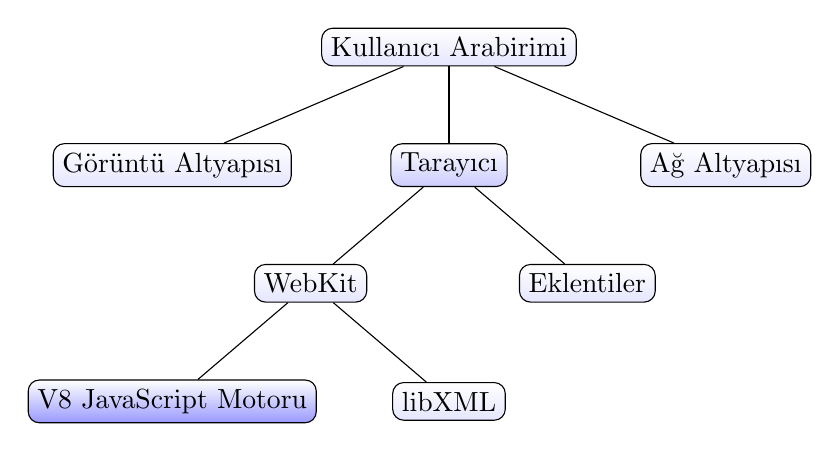
\begin{tikzpicture}[sibling distance=10em,
  every node/.style = {shape=rectangle, rounded corners,
    draw, align=center,
    top color=white, bottom color=blue!10}]]
  \node {Kullanıcı Arabirimi}
    child { node {Görüntü Altyapısı} }
    child { node[bottom color=blue!20] {Tarayıcı}
      child { node {WebKit}
        child { node[bottom color=blue!40] {V8 JavaScript Motoru} }
        child { node {libXML} }
      }
      child { node {Eklentiler} }
    }
    child { node {Ağ Altyapısı} };
\end{tikzpicture}
\uncover<2->{Diğerleri: Carakan - Opera, SpiderMonkey - Firefox, Chakra - Edge}
\end{frame}
% ----------------
\subsection{Dil Yapısı}
% ----------------
\begin{frame}[fragile]{Genel Görünüm}
\begin{columns}[T] % align columns

\begin{column}{.68\textwidth}
% \rule{\linewidth}{0.5pt}
\centering
\begin{minted}[fontsize=\tiny, bgcolor=DarkGray, linenos]{javascript}
    var degisken = 'javascript';
    function test(degisken) {
        for (var i = 0; i < 5; i++) {
            console.log(degisken + i);
        };
    };
    test(degisken);
    var nesne = {
        sayi  : 5,
        metod : function () {
            return this.sayi + 5
        },
        dizi  : [1, "pi", 3.14]
    };
    console.log(nesne.sayi);
    console.log(nesne.metod());
    console.log(nesne.dizi[1] + " sayisi: ", nesne.dizi[2]);
    console.log(nesne.olmayan_eleman);
\end{minted}
\end{column}%

\begin{column}{.28\textwidth}
Sonuç
\rule{\linewidth}{0.5pt}
\begin{minted}[fontsize=\tiny, bgcolor=DarkGray]{javascript}
javascript0
javascript1
javascript2
javascript3
javascript4
5
10
pi sayisi: 3.14
undefined
\end{minted}
\end{column}%

\end{columns}

\end{frame}
% ----------------
\begin{frame}[fragile]{\ttfamily{undefined}, \ttfamily{null} ve \ttfamily{NaN}}
\begin{columns}[T] % align columns

\begin{column}{.42\textwidth}
\centering
\begin{minted}[fontsize=\tiny, bgcolor=DarkGray, linenos]{javascript}
birdegisken
var birdegisken = null; birdegisken
typeof null
typeof undefined
null === undefined
null == undefined
NaN === NaN
Number.NaN === NaN
isNaN(NaN)
isNaN(Number.NaN)
\end{minted}
\end{column}%

\begin{column}{.54\textwidth}
\begin{minted}[fontsize=\tiny, bgcolor=DarkGray]{javascript}
"ReferenceError: birdegisken is not defined"
null
object // ECMAScript tanım hatası, doğrusu null
undefined
false
true
false
false
true
true
\end{minted}
\end{column}%

\end{columns}

\end{frame}
% ----------------
\begin{frame}[fragile]{Veri Tipleri/Operatörler}
\begin{columns}[T] % align columns

\begin{column}{.58\textwidth}
\centering
\begin{minted}[fontsize=\tiny, bgcolor=DarkGray, linenos]{javascript}
// Sayılar (Numbers)
2.998e8
100 + 4 * 11
(100 + 4) * 11

// Karakter Dizisi (Strings)
"Merhaba Dünya"
"Merhaba\nDünya"

"Merhaba" + "Dü" + "nya"

// Mantıksal (Boolean)
3 > 1
5 != 5
"a" == "b"

// Nesneler (Objects) Herşey
a = { b: 5, c: 4 }
a.b + a.c

// Diziler (Arrays)
a = [1, "test", 3, function(){ return "hello"; }, 5]
a[3]()
\end{minted}
\end{column}%

\begin{column}{.38\textwidth}
\begin{minted}[fontsize=\tiny, bgcolor=DarkGray]{javascript}
// 2.998 x 108 = 299,800,000
299800000
144
1144


Merhaba Dünya
Merhaba
Dünya
Merhaba Dünya


true
false
true


Object {b: 5, c: 4}
9


[1, "test", 3, function a(), 5]
"hello"
\end{minted}
\end{column}%

\end{columns}

\end{frame}
% ----------------

\begin{frame}[fragile]{Şartlı Çalıştırma/Döngüler}
\begin{columns}[T] % align columns

\begin{column}{.68\textwidth}
\centering
\begin{minted}[fontsize=\tiny, bgcolor=DarkGray, linenos]{javascript}
// If
var sayi = 50;
if (sayi < 10)
  console.log("Kücük");
else if (sayi < 100)
  console.log("Orta");
else
  console.log("Buyuk");

// While
var sayi = 0;
while (sayi <= 4) {
  console.log(sayi);
  sayi = sayi + 2;
};

// For
for (var sayi = 0; sayi <= 4; sayi++)
  console.log(sayi);
\end{minted}
\end{column}%

\begin{column}{.28\textwidth}
\begin{minted}[fontsize=\tiny, bgcolor=DarkGray]{javascript}
// If
Orta

// While
0
2
4
6

// For
0
1
2
3
4
\end{minted}
\end{column}%

\end{columns}
\end{frame}
% ----------------
\begin{frame}[fragile]{Fonksiyonlar/Prototipler}
\begin{columns}[T] % align columns

\begin{column}{.58\textwidth}
\centering
\begin{minted}[fontsize=\tiny, bgcolor=DarkGray, linenos]{javascript}
// Asal sayı kontrolü
function asalmi(sayi) {
    for(var i = 2; i < sayi; i++) {
        if(sayi % i === 0) {
            return false;
        }
    }
    return sayi > 1;
}
console.log(asalmi(7));
console.log(asalmi(12));
console.log(asalmi(15487457));

// Prototipler
var a = 7;
console.log(typeof a);

Number.prototype.asalmi = function(){
    return asalmi(this);
}

console.log(a.asalmi());
\end{minted}
\end{column}%

\begin{column}{.38\textwidth}
\begin{minted}[fontsize=\tiny, bgcolor=DarkGray]{javascript}
true    //<-- asalmi(7)
false   //<-- asalmi(12)
true    //<-- asalmi(15487457)
number  //<-- typeof a
true    //<-- a.asalmi()
\end{minted}
\end{column}%

\end{columns}
\end{frame}
% ----------------
\begin{frame}[fragile]{Kapsam (Scope)}{\ttfamily{var} neden önemli?}
\begin{columns}[T] % align columns

\begin{column}{.28\textwidth}
\centering
\begin{minted}[fontsize=\tiny, bgcolor=DarkGray, linenos]{javascript}
var x = "disarisi";

var f1 = function() {
  var x = "f1in icinde";
};
f1();
console.log(x);

var f2 = function() {
  x = "f2nin icinde";
};
f2();
console.log(x);
\end{minted}
\end{column}%

\begin{column}{.68\textwidth}
\begin{minted}[fontsize=\tiny, bgcolor=DarkGray]{javascript}
disarisi
f2nin icinde
\end{minted}
\uncover<2->{
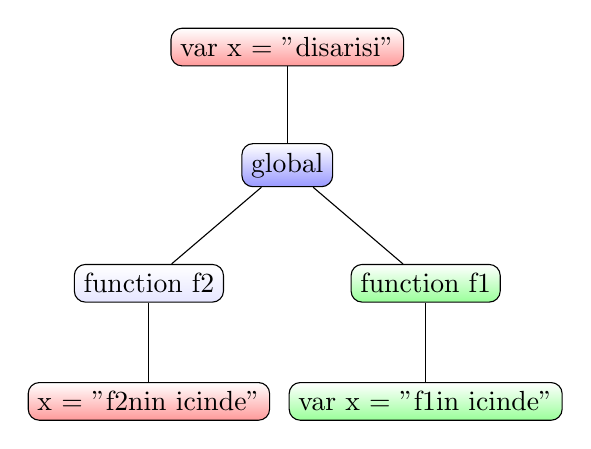
\begin{tikzpicture}[sibling distance=10em,
  every node/.style = {shape=rectangle, rounded corners,
    draw, align=center,
    top color=white, bottom color=blue!10}]]
  \node[bottom color=red!40] {var x = "disarisi"}
    child { node[bottom color=blue!40] {global}
        child { node {function f2}
            child { node[bottom color=red!40] {x = "f2nin icinde"} }
        }
        child { node[bottom color=green!40] {function f1}
            child { node[bottom color=green!40] {var x = "f1in icinde"} }
        }
    };
\end{tikzpicture}
}
\end{column}%

\end{columns}
\end{frame}
% ----------------
\begin{frame}{Sorular?}
\centering\pgfuseimage{js}
\end{frame}

\section{Node.js}

\subsection{Hikaye}

\begin{frame}
\centering\pgfuseimage{nodejs}
\end{frame}

% ----------------
\begin{frame}{Hikaye}{JavaScript'i Tarayıcıdan Çıkartalım}
\begin{itemize}
    \item {
        Sunucu tarafında web uygulamaları için geliştirilmiş bir
        çalıştırma ortamı. Açık Kaynak kodlu ve hali hazırda birçok
        platform tarafından destekleniyor (Linux, Mac OS X, Windows, Unix, BSD* etc.)
        \pause
    }
    \item {
        Ryan Dahl tarafından 2009 yılında geliştirilmeye başlandı.
        Şu anda Node.js vakfı tarafından finanse ediliyor ve Linux Vakfı'nın da
        üye kuruluşları arasında.
        \pause
    }
    \item {
        JS yorumlamak için Google'ın Chrome ile birlikte geliştirdiği V8
        JavaScript motorunu kullanıyor.
        \pause
    }
    \item {
        C, C++ ve JavaScript ile geliştiriliyor, kendi paket yönetim sistemi NPM
        (Node Package Manager) 'de 250.000'e yakın paket bulunmakta.
        \href{https://npmjs.com}{NPM}
    }
\end{itemize}
\end{frame}

\begin{frame}
    \centering\pgfuseimage{npm}
\end{frame}

\subsection{Peki Nasıl?}

% ----------------
\begin{frame}{Peki Nasıl?}
\begin{itemize}
    \item {
        Node.js tekil iş parçacıkları (threads) üzerinde çalışabiliyor fakat
        eşsamansız girdi/çıktı hareketlerine olanak sağlayan bir altyapıya dayanır.
        \pause
    }
    \item {
        Temeldeki en önemli bileşen tüm platformlara destek veren \textbf{libuv} kitaplığı.
        \textbf{libuv} ile işletim sisteminin ve dosya sisteminin olanaklarını
        kullanarak eşzamansız bir akış döngüsü (event loop) yaratılır.
        \pause
    }
    \item {
        Tekil bir akış döngüsü iş listesinde birşeyler olduğu sürece çalışmaya devam eder.
        \pause
    }
\end{itemize}
\end{frame}

\begin{frame}{Akış Döngüsü}
    \centering\pgfuseimage{node-loop}
\end{frame}

\begin{frame}[fragile]{Dosya Sistemi}
\centering
\begin{minted}[fontsize=\tiny, bgcolor=DarkGray, linenos]{javascript}
var fs = require('fs');
var sayi = undefined;

// birArttir fonksiyonu her çalıştırıldığında
// sayi.txt'nin içeriğindeki sayının bir fazlasını verecektir.

function birArttir() {
  fs.readFile('sayi.txt', function (err, dosyaIcerigi) {
    sayi = parseInt(dosyaIcerigi);
    sayi++;
  })
};

// çalıştırıldığında ekrana `undefined` basmasını bekleriz
// çünkü okuma işlemi eşzamansız bir işlem ve o işlem bitip
// ona parametre olarak verdiğimiz fonksiyonu
// çağırana kadar sayi `undefined` olmaya devam edecek.

birArttir();

console.log(sayi);
\end{minted}
\end{frame}
% ----------------

\begin{frame}{Basit bir Node.js Sunucusu}
    \centering\pgfuseimage{server}
\end{frame}

\begin{frame}{Kimler kullanıyor?}
\begin{itemize}
    \item {\href{https://koding.com}{Koding}}
    \item {\href{https://paypal.com}{PayPal}}
    \item {\href{https://uber.com}{Uber}}
    \item {\href{https://netflix.com}{Netflix}}
    \item {\href{https://linkedin.com}{LinkedIn}}
    \item {\href{https://microsoft.com}{Microsoft}}
    \item {\href{https://github.com/nodejs/node-v0.x-archive/wiki/Projects,-Applications,-and-Companies-Using-Node}{ve diğerleri...}}
\end{itemize}
\end{frame}

\begin{frame}{Sorular - Teşekkürler}
    \LARGE{{Gökmen Göksel - \url{gokmen@goksel.me}}}

\begin{itemize}
    \item {\href{https://gokmen.goksel.me}{gokmen.goksel.me}}
    \item {\href{https://github.com/gokmen}{github.com/gokmen}}
    \item {\href{https://twitter.com/gokmen}{twitter.com/gokmen}}
    \item {\href{https://speakerdeck.com/gokmen}{speakerdeck.com/gokmen}}
\end{itemize}
\end{frame}

\end{document}
% ----------------
